\apendice{Especificación de diseño}

\section{Introducción}

\section{Diseño de datos}
Dado que consideraba un factor muy importante la forma de tomas los datos, se explica este apartado detalladamente el aspectos relevantes.


\section{Diseño procedimental}
A continuación, se procede a explicar algunas nociones relevantes de cómo interactúan entre sí los diferentes elementos que conforman el proyecto. Dado que no es una aplicación al uso, sino que se compone de múltiples elementos, mostraré un diagrama de despliegue y un diagrama de secuencias.

\subsection{Diagrama de despliegue}
La estructura que ha acabado adoptando el proyecto puede resultar algo compleja, por lo que explicaré, en primer lugar, cómo está organizado \ref{fig:d_desp}.

Para empezar es muy importante aclarar que hay dos implementaciones del juego. Por un lado está el juego que recibirán los usuarios. El juego que reciben los usuarios es lo que consideraríamos un juego real, es decir, el jugador dispone del menú de inicio y banda sonora. Por el otro lado, tenemos el juego que va a utilizar el agente inteligente. Este juego no dispone de menú principal, la partida comienza directamente e intenta conectarse al \emph{socket}. La banda sonora se decidió retirar por comodidad a la hora de trabajar, ya que acababa resultando cargante.

Para la creación de los modelos los agentes inteligentes se han seguido dos vertientes principales. Una es la implementación de un decision tree, que es la que primero se probó. La otra vertiente el la relativa a los algoritmos evolutivos. Por este motivo ha dos bloques que, a priori, iban a ser completamente diferentes, pero acabaron siendo muy similares. A pesar de tener cierta similitud, esas pequeñas diferencias hicieron que conservase la estructura inicial.


\begin{figure}
    \centering
    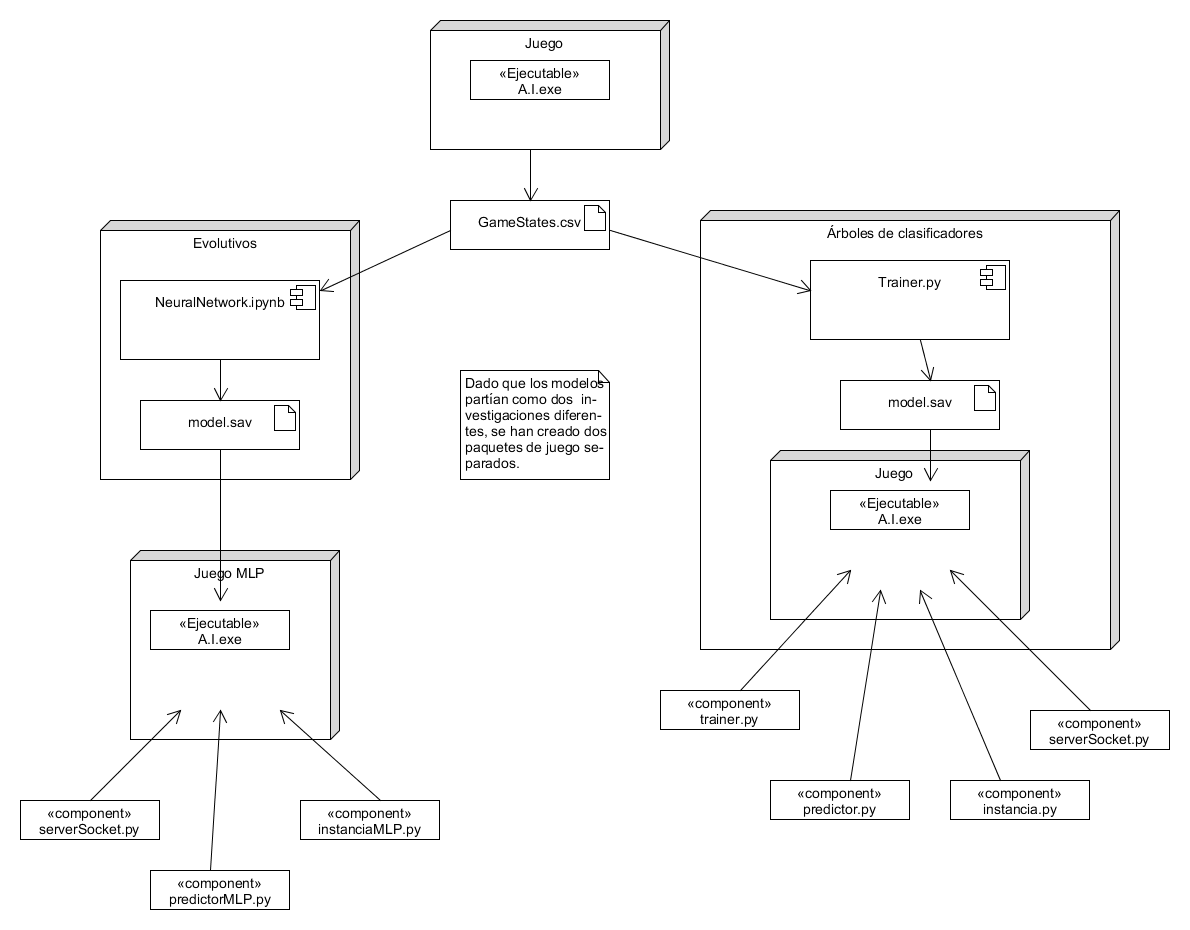
\includegraphics[width=\textwidth]{despliegue}
    \caption{Diagrama de despliegue}
    \label{fig:d_desp}
\end{figure}


\subsection {Diagrama de secuencias}
En esta sección se pretende aclarar el funcionamiento de, al menos, uno de los agentes, ya que el otro es muy similar.

El entrenamiento y explotación del modelo de agente inteligente se realizan tres acciones. La captura de datos, para el entrenamiento por imitación, en entrenamiento utilizando el clasificador preferido y, para finalizar, la utilización del modelo entrenado sobre el juego \ref{fig:d_sec}. 


\begin{figure}
    \centering
    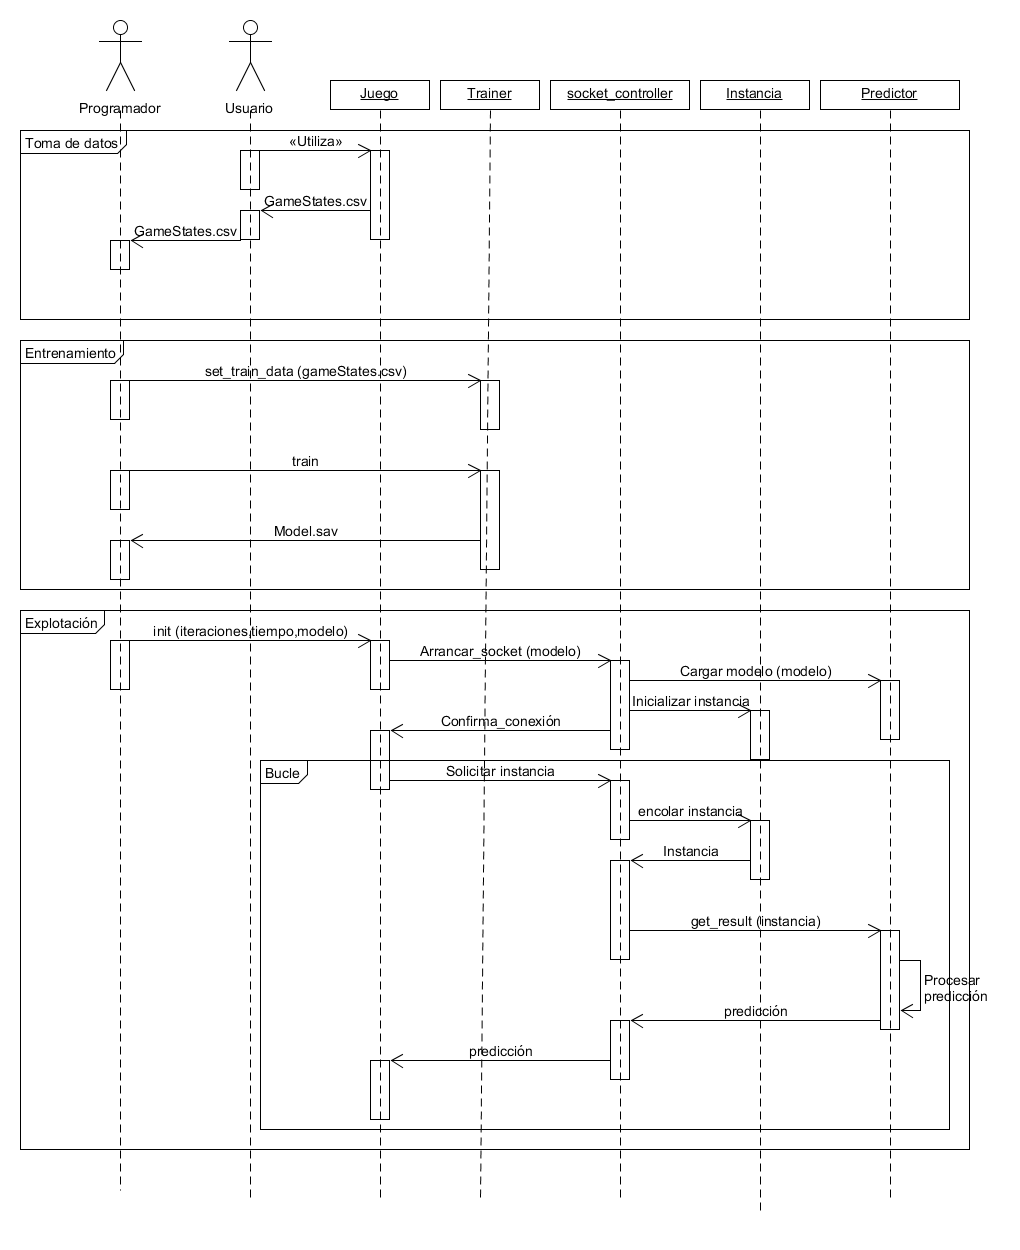
\includegraphics[width=\textwidth]{secuencias}
    \caption{Diagrama de secuencias (Arboles de decisión)}
    \label{fig:d_sec}
\end{figure}

La captura de datos es muy sencilla: el jugador utiliza el juego normalmente y el juego crea un «log» con todas las instancias que se han ido generando a lo largo del juego. EL usuario deberá enviar al programador los resultados de la captura de datos de la partida para que este pueda trabajar con ellos.

El entrenamiento es muy sencillo y se compone de dos pasos. En primer lugar decimos al entrenador qué fichero de datos queremos utilizar. A continuación, una vez ha procesado todos los datos, se le indica que inicie el entrenamiento. Como resultado deberíamos obtener un modelo entrenado.

La explotación del modelo entrenado ya es algo más sofisticada, aunque sigue siendo un flujo relativamente sencillo.
\begin{itemize}
    \item 1 - El programador lanza el juego, indicando por parámetro el numero de rondas, el tiempo máximo por ronda y el modelo que tiene que utilizar.
    \item 2 - En cuanto se lanza el juego, este ejecuta un script de \emph{Python} que abre, a su vez, un socket con el que establecer la comunicación entre el juego y el agente inteligente.
    \item 3 - El script de \emph{Python}, además de abrir el socket, carga el modelo e inicializa el procesador de instancias.
    \item 4 - Realizados estos pasos el socket confirma la conexión y se comienzan a mandas las instancias de juego a este.
    \item 5 - Dado que el procesado de instancia se va a hacer en «paquetes» de cuatro, por el concatenado de instancias que se explica en la memoria, lo primero que hace el socket al recibir la instancia es encolarla.
    \item 6 - Una vez encolada, el procesador de instancias la devuelve junto con las tres anteriores.
    \item 7 - La instancia procesada se envía al «predictor» y éste, después de procesar internamente la predicción, la devuelve al servido de socket.
    \item 8 - EL servidor de socket devuelve la predicción al juego, que realizará la acción correspondiente.
\end{itemize}

Este proceso de envío, procesado y predicción se hace en bucle hasta que el jugador muera o se cierre el juego. El bucle se realiza cuatro veces por segundo.


\subsection {Diagrama de clases}
A continuación se muestra el diagrama de clases. Considero que es un diagrama de clases «especial», ya que Unity3D no trabaja con las clases tipo java que podemos conocer, Unity3D trabaja con GameObjects que, a su vez están formados por una o varias clases de .net y otros tipos de objetos, incluso un GameObject puede no tener ninguna clase .net. Este hecho me ha dificultado el desarrollo del diagrama de clases. Finalmente he decidido crear yo mi propio tipo de diagrama para poder englobar las clases que todos conocemos y los GameObject de Unity3D.


\begin{figure}
    \centering
    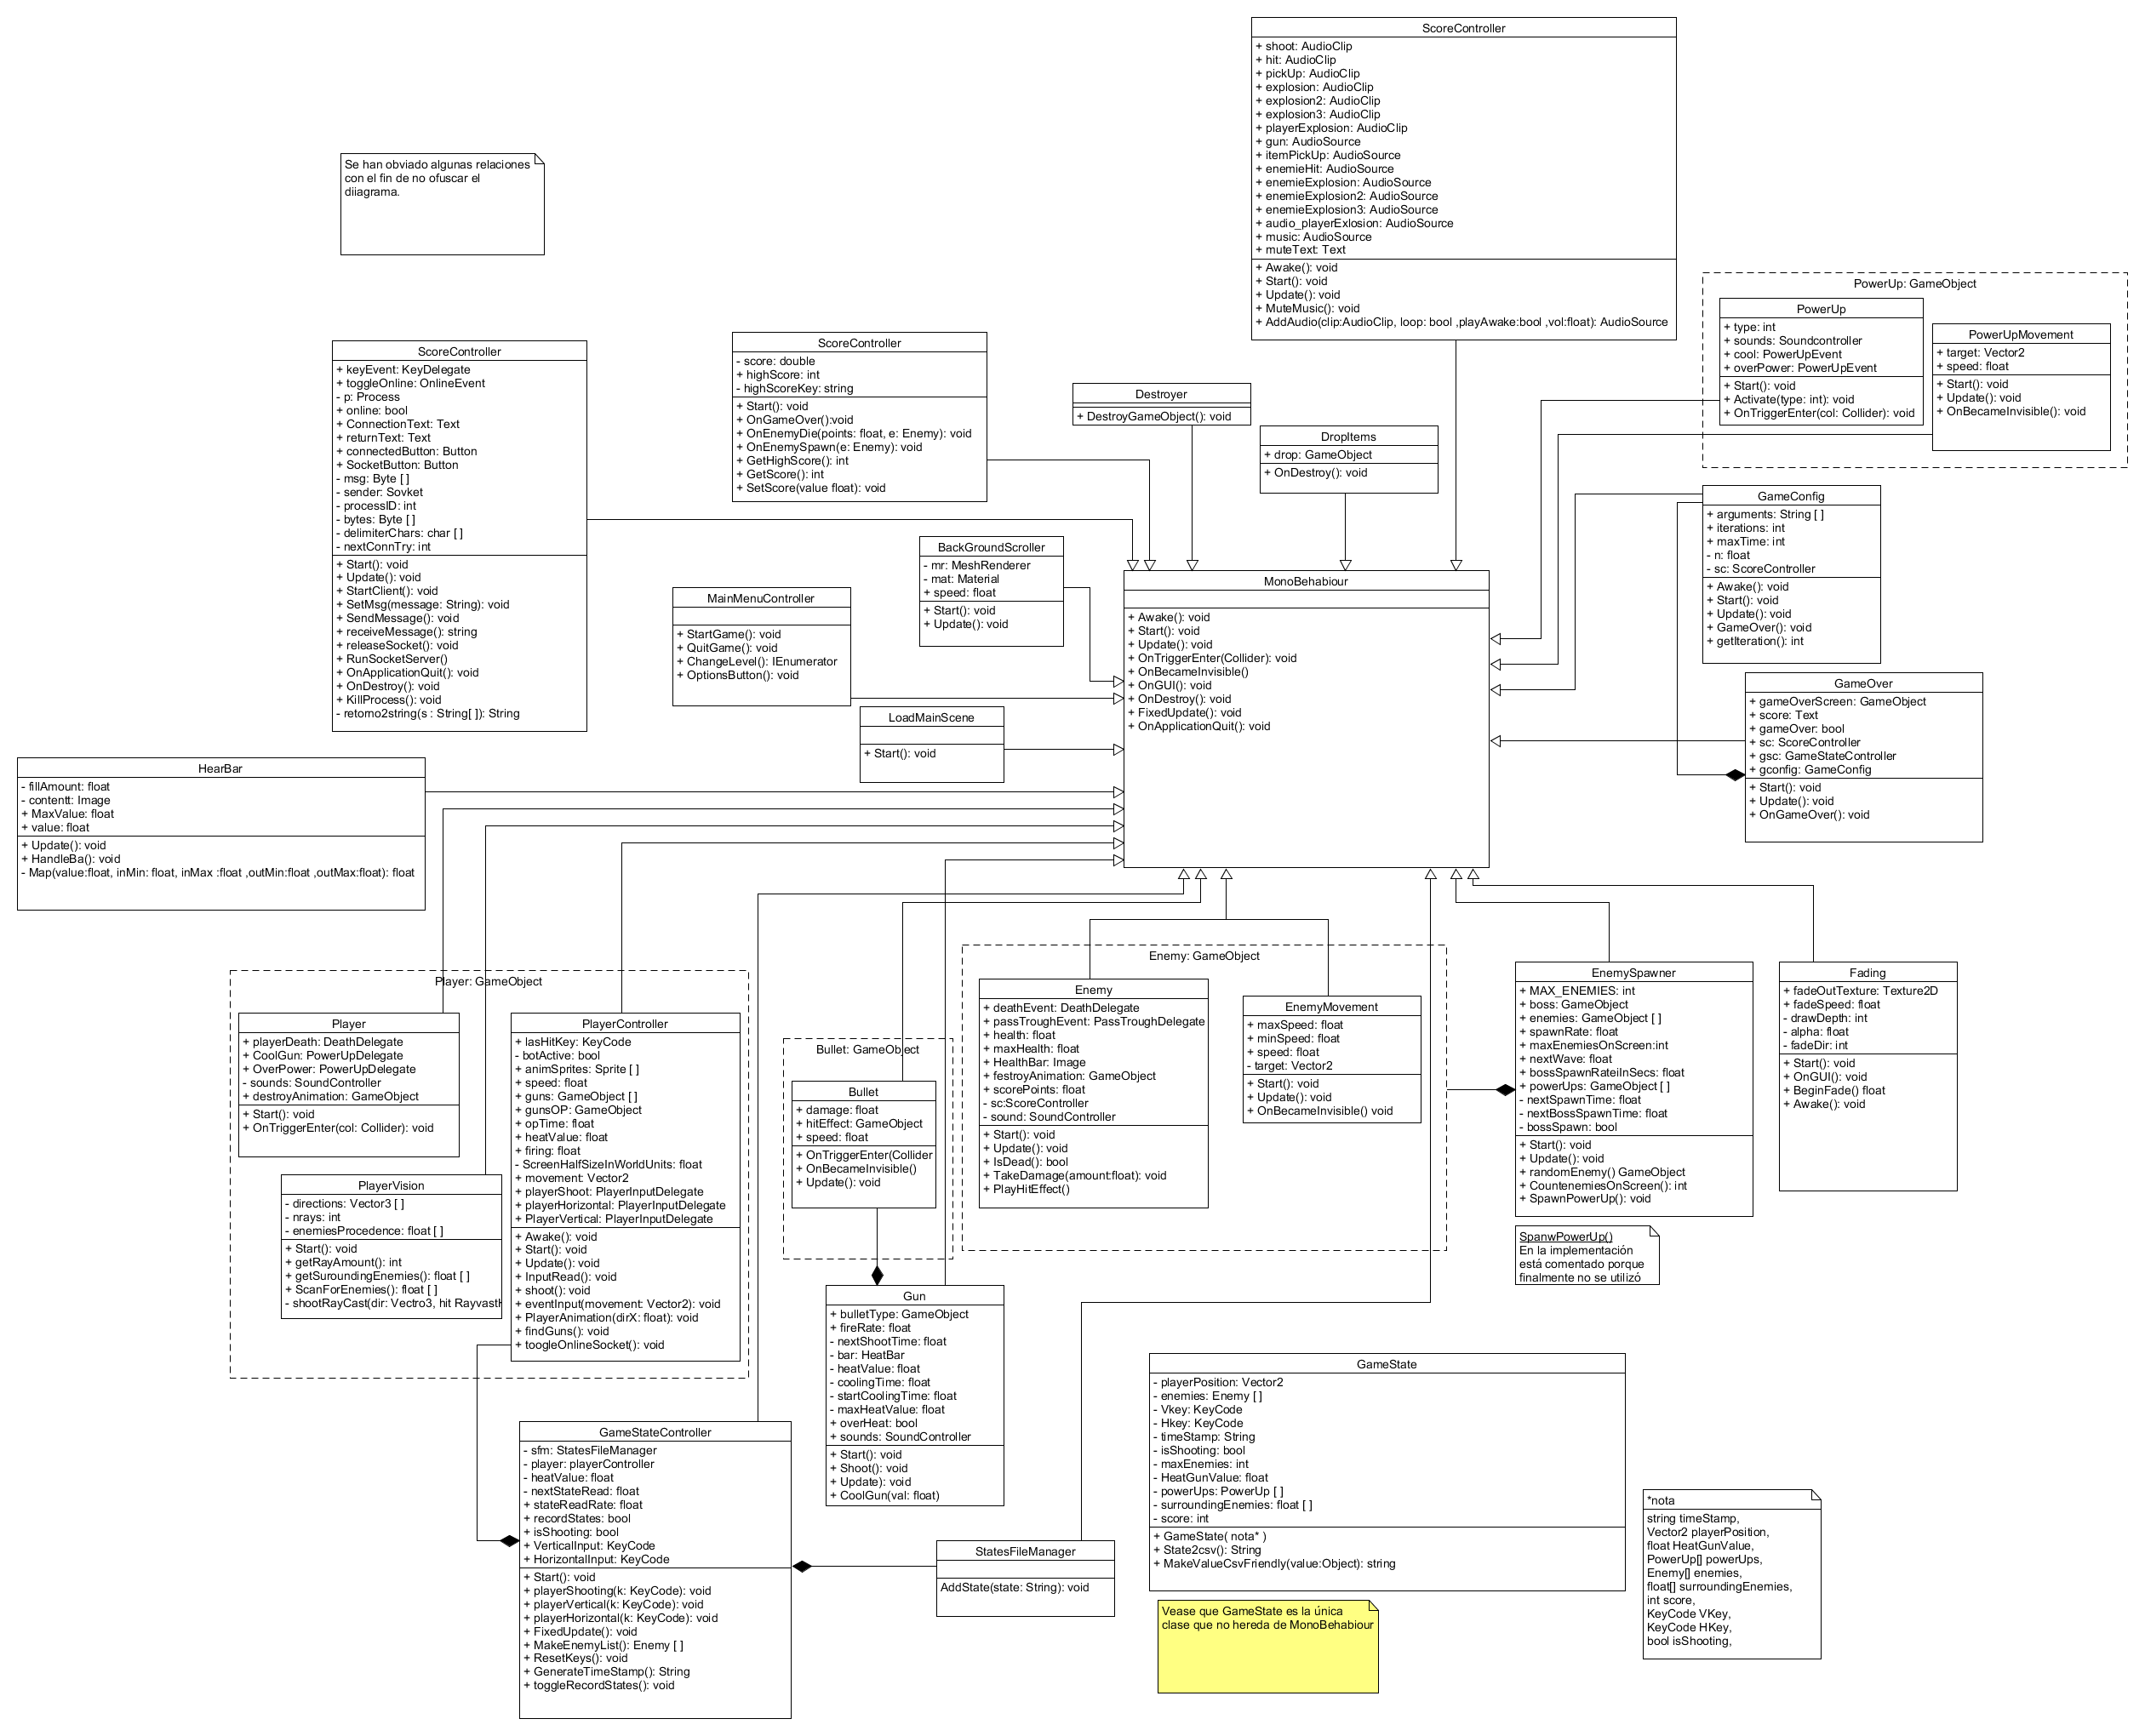
\includegraphics[width=\textwidth]{clases}
    \caption{Diagrama de clases}
    \label{fig:d_clases}
\end{figure}
